\chapter{The key concepts}

\section{Introduction -- random fields, a gentle introduction}
We have seen in the first chapter that many data structures have one thing in common--they life in space where there is spatial autocorrelation. This autocorrelation is reflected in a random field.

A spatial random field is a \textit{random variable}\index{random variable} that represents spatially continuous phenomena in 2 dimensions. Since this is a difficult concept to grasp this chapter slowly builds up to these by first considering simple univariate random variables familiar from basic statistics courses, then moving to 1-dimensional random fields and eventually the 2-dimensional random fields that will be prominent throughout this book.


\subsection{A simple univariate random variable}

\textit{Random variables} are a key concept in all statistical literature as they are the basic objects that are used in all statistical inference. Random variables are variables that are assumed to follow some probability distribution, i.e.\ they take on different values or values within a certain interval with different probabilities. 
% something on a discrete random variable
A very familiar example is a random variable that follows a normal distribution. This one-dimensional continuous random variable can take on any value, but values close to the mean are particularly likely, resulting in the famous bell curve. As an example lets assume that IQ values in a country are normally distributed with mean 100 and standard deviation 15. The probability density of this distribution is plotted in Figure \ref{fig:ch2:normal}, black line indicating that values around the mean rather likely and those further away are less likely. 

\begin{figure}
\centering
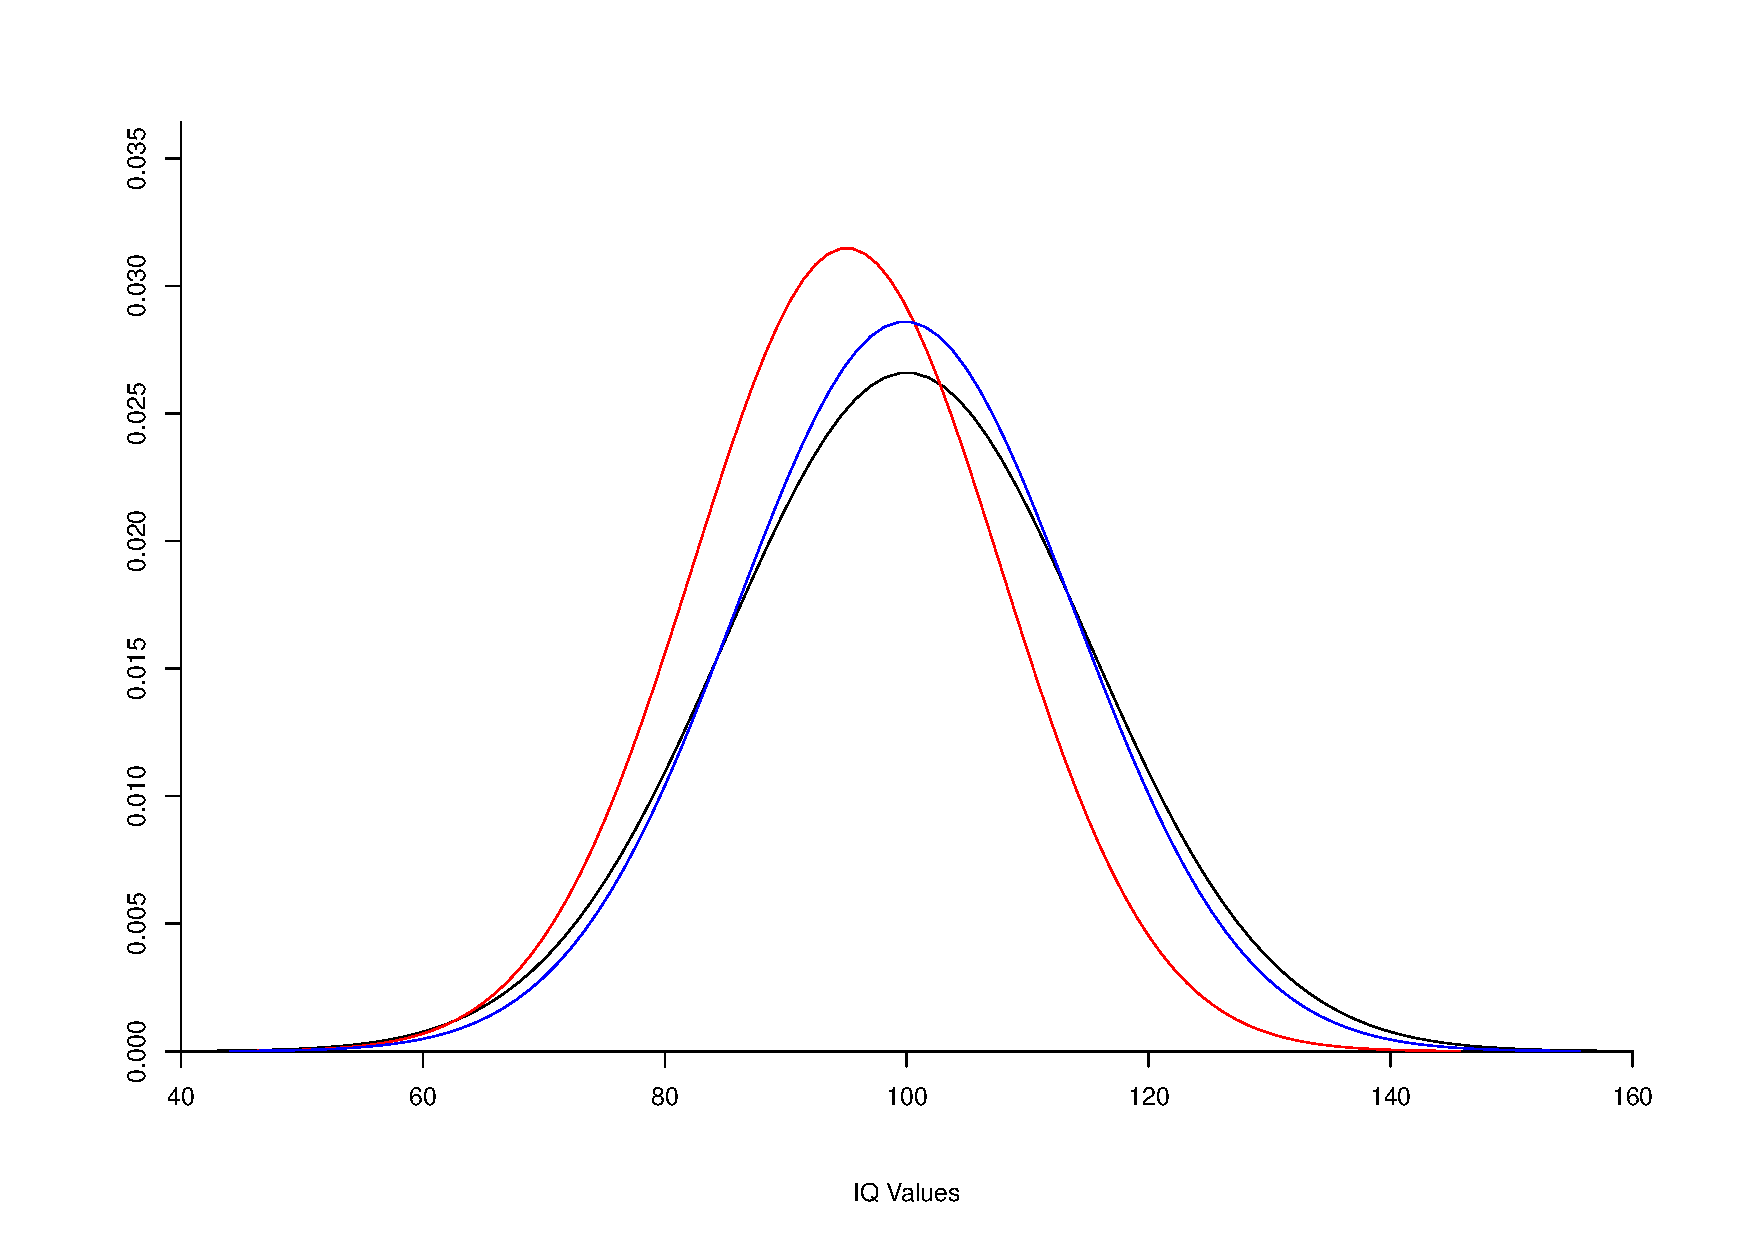
\includegraphics[width=0.5\textwidth]{normal_density}
\caption{\label{fig:ch2:normal} The probability density of the normal distribution with mean 100 and sd = 15 (black line), the density estimated from a sample of size 20 (red line) and the density estimated from a sample of size 200 (blue line). }
\end{figure}

In practice, we usually we do not know the true distribution for a given population but use a \textit{sample} to estimate the parameters of the distribution from this sample, for example using maximum likelihood estimation methods, as discussed in standard statistics textbooks. For the example in Figure \ref{fig:ch2:normal} a sample of size 20 resulted in an estimate of mean 95.03 and standard deviation 12.67; the estimated density is shown as the red line in the same figure. However, a much bigger sample of size 200 provided a much better estimate with a mean of 99.84 and standard deviation 13.95, represented by the blue line in Figure \ref{fig:ch2:normal}. This improvement in precision is not surprising as we gain more \textit{independent information} on a population from a sample of a bigger size and hence our estimates become more precise. 

An important point here is that typical estimation and inference approaches assume that any sample consists of \textbf{independent observations} or \textbf{replicates}.  Dependent samples are likely to tend to be similar and hence to not provide much new information on the population. This will eventually introduce bias.  In practice, this implies that observations have to be made independently of each other, and the assumption is made that there are no similarities or relationships among any of the observations that might result from the sampling process. For instance, for the estimation of IQ values in a country one would have to sample across the population and not just from a specific subgroup  of the population, say university students, as this would bias the estimation. In this case there is a similarity or relationship among the resulting observations as the observation have all be been made from members of the same subgroup.
We will see further below that in the central concept of the book--in random fields there is no assumption of independence among measurements; they are explicitly assumed to show \textbf{systematic dependence} among measurements and specific  assumption is made about the nature of this dependence. We will start thinking about this dependence in the next section. We will initially look at a one dimensional random field even though most of the random fields discussed in this book are spatial random fields, i.e.\ random fields in 2D.

\subsection{A random field in 1D}
Random field in !D is a random variable that the realisations of which take on values in one-dimensional space. Lets think about this through an example. Say, the 25 children in a primary school class in Helsinki are set to learn about temperatures, its measurement and how it fluctuates on their home town during a day in spring. In other words the random variable of interest is ``temperature throughout school day in spring in Helsinki''. Continuous in time. To estimate this random variable on one specific day in May, they the children are each given a different random time between 8:00 am and 4:00 pm by their teacher and are asked to check and write down the temperature at the thermometer in their classroom that measures the outside temperature at exactly that time. 

When comparing these data to the IQ data we discussed earlier we realise a number of things. Clearly, these temperature measurements are \textit{not independent}--it is likely that the measurements taken at as 12:45 and at 12:46 are not very different from each other. The measurements tell us about the temperature throughout a specific school day in one place in Helsinki, but they do not tell us much about the temperature and its fluctuations elsewhere in the country or the world. Even if each child was given two random times to measure the temperature and the number of observations was doubled, these would not improve our knowledge about the temperature levels and fluctuations that day elsewhere.

However, this is not what the children where meant to learn anyway --they were meant to get a picture of the behaviour of temperature throughout a day in spring in Helsinki.  Now, they have only measured it at some points in time, not continuously through time.
However, if one makes some general reasonable assumptions about how temperature behaves over time, it is possible to get an idea of the temperature at times when the temperature has not been measured, based on the given values. 
%Figure \ref{fig:ch2:1D} shows an example of this [bad figure]. 
Intuitively, one would want to assume 
\begin{itemize}
\item[a)] that temperature values measured within a few minutes of each other are similar to each other,  
\item[b)] that the temperature does not jump to some high value and back down frequently between measurements. 
\end{itemize}

With these simple assumptions one could just  connect the observations by straight line, as in Figure \ref{fig:ch2:1D}; doing this means we are simply taking the average between the values. But we know that temperature does not behave like this and that it is more smooth. Hence we would like some smooth function to describe the relationship between two observations--and this smooth function depends on distance between the observations and describes their similarity.

Note that the temperatures in this example have only been observed on one single day, while there is an interest in temperatures in Helsinki in spring. This is inplies  Values would be different if different day was chosen. 
%Also, if different times for measuring the 
only one realisation.


While the school children in Helsinki could probably repeat the measurement procedure on several  --randomly chosen-- days throughout spring, in many realistic examples This has important consequences 

Note that measured only at very few points
and this realisation has not been fully observed

This is what a random field in 1D does, make assumptions on this functional form
random variable 





Note there is actually another set of assumptions at work here- one that concerns the measuring process.
\begin{itemize}
\item[c)] that temperature is measured at different times during the day and year and month  
\item[d)] and that the person does not get into their car more frequently when it is warmer outside than when it is cold.
\end{itemize}
[example does not work very well; fewer values during the night, but wanted non-regular measurements that one would get from some measurement device...]



With these assumption we implicitly make assumptions about the nature of the dependence among the observations.

% besseres Beispiel finden
% figure showing continuous values
% values measured
% crosses at times when we would like to interpolate

\begin{figure}
\centering
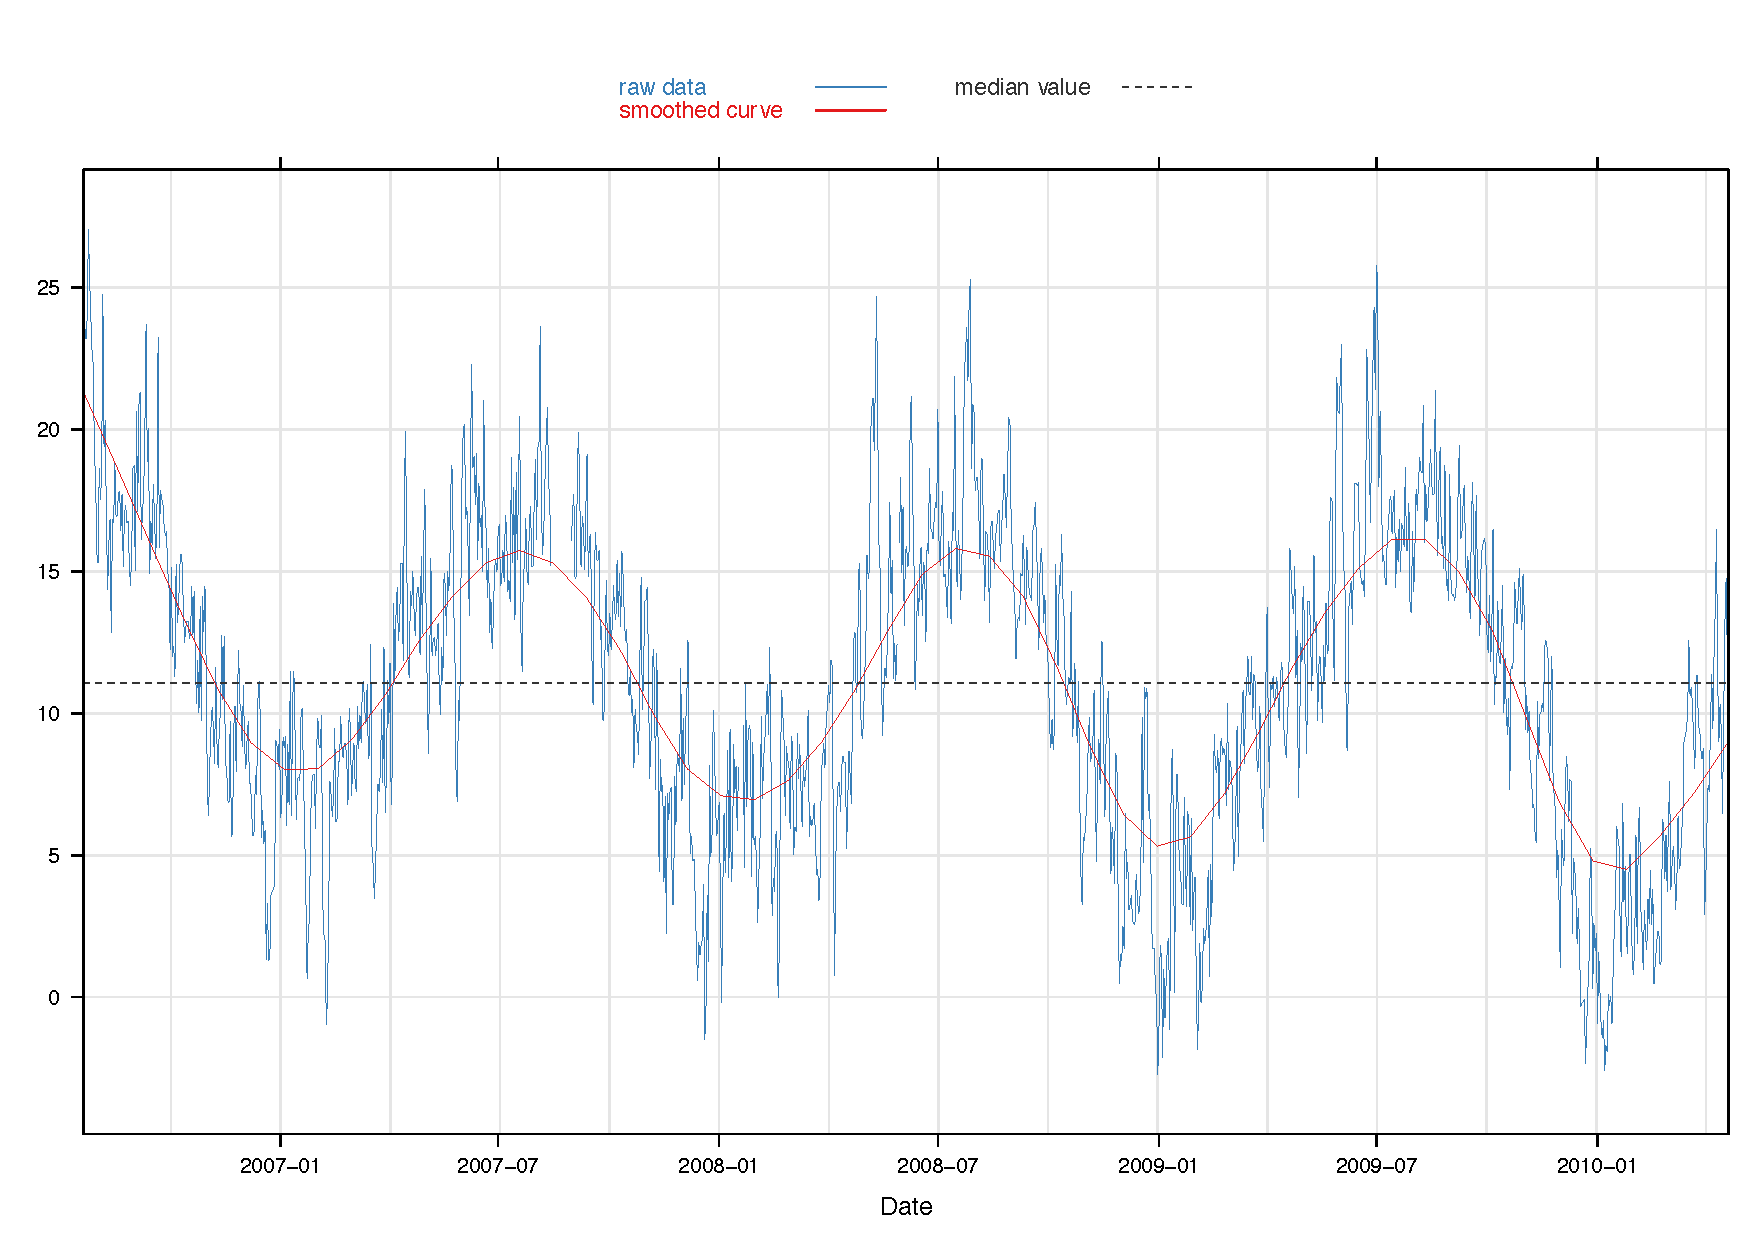
\includegraphics[width=0.5\textwidth]{temp_timeseries}
\caption{\label{fig:ch2:1D} Temperature over time... this is a bad plot....}
\end{figure}

\begin{itemize}
\item realise that observations are not independent through time
\item prediction hence needs to take the other values into account 
\item interpolated values should, on average, be similar to all values measured
\item interpolated values should be similar to values measured close in time
\end{itemize}



random field has properties that describe average behaviour and on distance in time


\subsection{The same thing in 2D}
Lets now move to 2 dimensional space. 

key points:
\begin{itemize}
\item realise that observations are not independent through space
\item interpolated values should, on average, be similar to all values measured
\item interpolated values should be similar values close in space
\end{itemize}

\section{Random fields -- and how they appear everywhere}

Lets have a look at a few examples of data structures.

\subsection{Spatially continuous data as random fields}

\subsection{Spatial point processes, conditional on random fields}

\subsection{Transect data thinned spatial point processes, conditional on random fields}

\section{Random fields -- technical definition}

